\chapter{Prototype}
\label{chapter:prototype}

\section{Overview}

The basic approach works in five steps: filter, root mean square (RMS) calculation, gate, gain adaption, delay.\\
The processing chain starts with a low-cut and a high-shelf filter which will be applied sample wise on the incoming audio. These filters are a simplified mapping of the perception of sound pressure for human beings. This is the first step to adjust the plug-in to loudness instead of sound pressure (as done in FOOTNTE). However, the plug-in won’t be running with the full loudness detection algorithm (FUTNOT) due to calculation time and real time capability (see SPÄTER? oder hier?).\\
After the filter section every sample is passed to the RMS calculation.  The goal is to output the squared average of a previously specified period of time. The square root will be determined in the following calculation of the equivalent dB value. The plug-in converts the linear audio samples into the logarithmic dB scale in order to display gain values and loudness goal (see gain part?) in dB in the user interface (UI) as it is the standard scale of DAWs. Thereby the executive sound engineer will intuitively know how to interpret and interact with the UI (see design part?).\\
When the dB conversion is done, all the samples pass through an initially specified gate. The gate will set all samples with lower dB value as its threshold to the current loudness goal (see gain, see improve). In this way the plug-in will not operate when it is fed with silence or irrelevant noise.\\
Next step after the gate is the gain adaption. In this step the gated RMS value is compared to the current loudness goal. Depending on the difference of both values it will result in an preliminary gain. The gain variations per sample are smoothed comparable to the RMS calculation. This leads to the final gain value.\\
Lastly the new gain is multiplied with the current sample. Because the plugins behaviour is smoothed as it shall sound natural, it will not react instantly to the input. To compensate the reaction time it delays the input signal before multiplying the calculated gain. This delay is later offset by the DAW.\\ 
During development most of the parameters described in the following sections were settable in a basic dummy UI. This was realised with the standard JUCE slider and button objects and used for tests and fast adjustments.\\

\begin{figure}
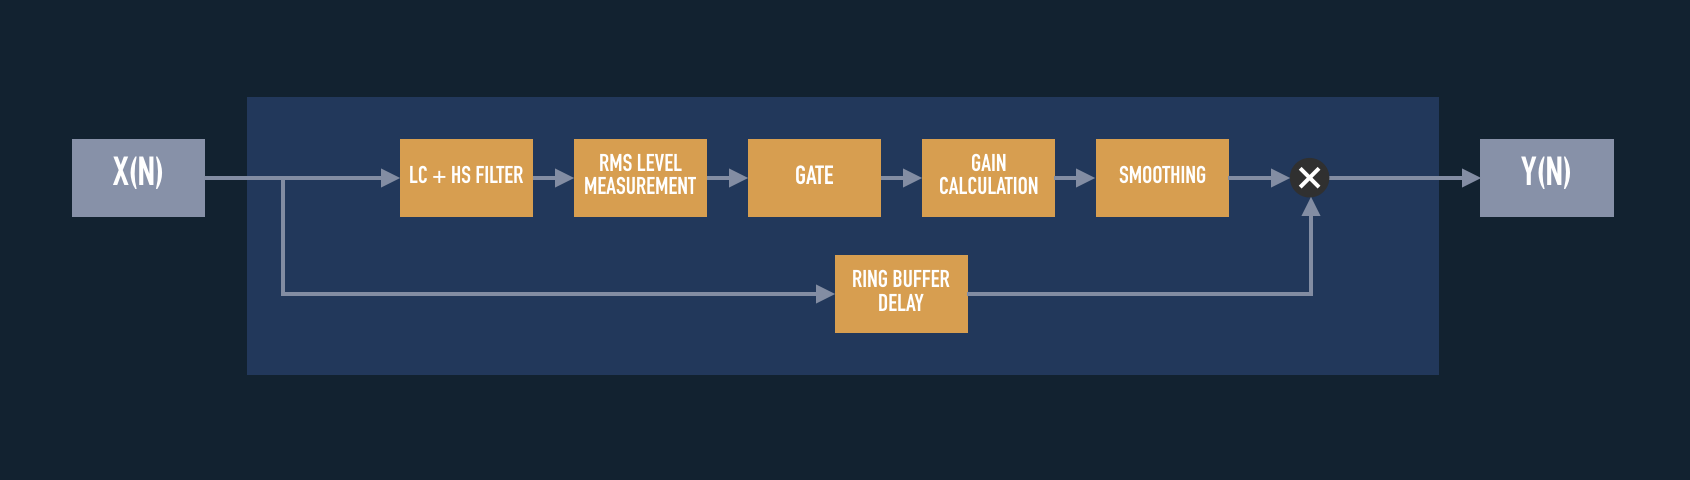
\includegraphics[width=\textwidth]{images/chain01}
\caption{Prototype processing chain}
\end{figure}

\section{Filter}

While gathering information on how to improve my idea of the plug-in I got interested in the ITU-R BS.1770-4 [FOOTNOTE pls] algorithm. It classifies an audio file for its humanly perceived loudness. The main use of this algorithm is found in television and music streaming services as they can keep the program loudness steady while switching content. As the human perception is also of interest for mixing a song, I examined how it was done. Due to a good documentation about how to implement the loudness algorithm I build a copy of it in python and decided which elements I would adopt in my plug-in. The first elements were the two filters. Like described above, their use is to mimic the human perception of sound pressure at different frequencies. The first filter is a low cut for the reason that human hearing is insensitive to low frequencies. The second filter is a high shelf and is ”used to account for the acoustic effects of the head” [wie zitiert man]. This imitation of the human hearing is greatly simplified but cost effective in terms of computation. The low cut filter has a cutoff frequency at 38 Hz, the high shelf around 1681 Hz. They are initialised at every plug-in startup in the JUCE method “prepareToPlay” with the current sample rate of the integrating DAW:\\

\lstset{language=C++}
\begin{lstlisting}[frame=single]
lowcut.setCoefficients(38.0, sampleRate, (1.0/2.0));
highshelf.setCoefficientsShelf(1681.0, sampleRate, 4.0);
\end{lstlisting}

The implementation is based on the biquad filter from the Book BLA (BLA NOTE auch im code).  I have chosen the second order biquad filter architecture as it is a very flexible and simple solution with just two samples delay. The calculation of filter coefficients is adopted as follows:

$f_c = $ cut-off frequency, $f_s = $ sampling frequency (rate), $K = tan(\pi f_{c}/f_{s})$,\\
$Q = $ factor for height of the resonance, $G = $ gain, $V_0 = 10^{G/20}$

\textbf{Lowcut:}\\
$b_0 = \frac{Q}{K^{2}Q+K+Q}$ \tab $b_1 = -\frac{2Q}{K^{2}Q+K+Q}$ \tab $b_2 = b_0$\\
$a_1 = \frac{2Q*(K^{2}-1)}{K^{2}Q+K+Q}$ \tab $a_2 = \frac{K^{2}Q-K+Q}{K^{2}Q+K+Q}$

\textbf{Highshelf:}\\
$b_0 = \frac{V_0+\sqrt{2V_0}K+K2}{1+\sqrt{2}K+K^2}$ \tab[0.4cm] $b_1 = -\frac{2(K^2-V_0)}{1+\sqrt{2}K+K^2}$ \tab $b_2 = \frac{V_0-\sqrt{2V_0}K+K2}{1+\sqrt{2}K+K^2}$\\
$a_1 = \frac{2(K^2-1)}{1+\sqrt{2}K+K^2}$ \tab $a_2 = \frac{1-\sqrt{2}K+K^2}{1+\sqrt{2}K+K^2}$\\

Hence the loudness algorithm uses second order filters (with two delay memories) it works like this:

Biquadfilter Bild

It is the same as my implementation in the Filter class:\\

\begin{lstlisting}[frame=single]
double AutoVocalCtrlFilter::process(double sample)
{
    const double mid = sample - a1 * z_1 - a2 * z_2;
    const double out = b0 * mid + b1 * z_1 + b2 * z_2;
    
    z_2 = z_1;
    z_1 = mid;
    
    return out;
}
\end{lstlisting}

Before implementing in C++ I testen my filter class in python. Therefor I send different signals with frequencies between 0 and 20000Hz through both filters and plotted the resulting amplitudes in a graph via pyplot(alter fußnoten verweis?). The current algorithm results in a descent graph (Fig. 3.2 NOCH ÄNDERN). To test the C++ version of the filter I compared the results of the same input with the previously tested python implementation.\\
The implementation is capable of many filter styles at different cutoff frequencies. For my plug-in it is used for the low cut and high shelf filter described above, which are simply processed one after the other on the current audio sample for each channel Wie VIELE AM ENDE??:\\
\begin{figure}
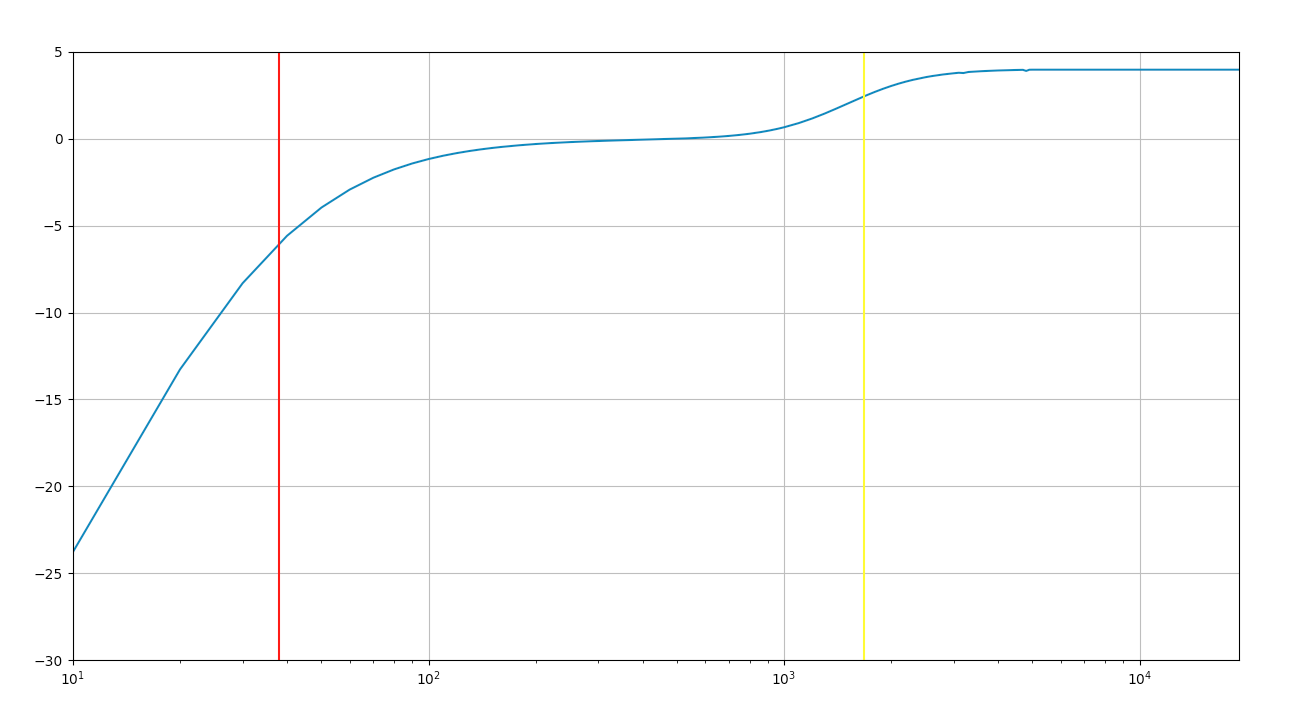
\includegraphics[width=\textwidth]{images/filter_test}
\caption{Plotted filter test}
\end{figure}

\begin{lstlisting}[frame=single]
double updateFilterSample(double sample, AutoVocalCtrlFilter hs,
AutoVocalCtrlFilter lc)
{
    return hs.process(lc.process(sample));
}
\end{lstlisting}

The updateFilterSample method returned the filtered samples for further processing.\\

\section{RMS}

To measure the level of the audio signal at the current position the plug-in calculates a root mean square (RMS) value of the last XX ms. This means it is calculating the root of the average from the squares of each sample in the set time window.\\
It uses RMS calculation because it is part of the imitation of human perception and because it has the necessary time to calculate an average value as it does not need to react fast. A human will (F. A. Everest, The Master Handbook of Acoustics, New York: McGraw-Hill, 2001.) not interpret a small impulse of a handful of samples as loud as a audio signal at the same level of longer duration.  For example “a 3-msec pulse must have a level about 15 dB higher to sound as loud as a 0.5-sec (500-msec) pulse”. This is also part of the BLABLA loudness standard. Additionally the “RMS is equal to the value of the direct current that would produce the same average power in a resistive load” [wikipdia].\\
The RMS implementation is based on the Book Digital Audio Signal Processing by Udo Zölzer (123) and can be performed in one line of code:\\

\begin{lstlisting}[frame=single]
double updateRMS2(double sample, double last, double co)
{
    return (1. - co) * last + co * (sample * sample);
}
\end{lstlisting}

The already filtered samples are used for this calculation and the result is written into the rms2 vector. The Co parameter is a time coefficient (see gleich) of small size. This parameter influences the weight on how much the current squared sample will inflict the quadratic mean. In normal RMS procedure the final result is the square root of the value the plugin results in. In this case we can skip the calulation because it will be converted into the logarithmic dB scale in the next step and a square just changes the value of one coefficient in this process. The final RMS value will only appear as logarithmic dB but save a little time.\\

\section{Time Coefficients}

The time coefficients are used for RMS calculation and to realise the compress and expand times (see later). They are determined with a formula by Udo Zölzer (quell):

$$1.f - \exp(-2.2*(1./currentSampleRate)/(ms/1000.))$$
$$=  1.f - \exp(-2.2*(1./currentSampleRate)/s)$$

Udo Zölzer decided to use the exponential function because it draws a natural decay. He determined -2.2 for the first part in the exponent by solving an equation system to achieve an attack time MATHE ta = t90 - t10. This means that when a calculation similar to the RMS calculation defined above uses such an time coefficient, its reaction on a input change will need the chosen amount of time to get from 10% of the final reaction to 90%. Illustrated in Fig.SIEHE UNTEN.
The second part in the exponent (1./currentSampleRate)/s) calculates the proportion of one sample to the amount of seconds of the MATH ta. This needs to be done because it will be used on every sample.

BILD MIT ATTACK ZEIT ODER RMS MITTEL DURCH IMPLUSE VERÄNDERUNG t90 und t10\\

\section{Gate}

The plug-in should operate while there are vocals and stop if there are none or just a soft decay. Else it would produce unwanted effects by amplifying noise. Additionally it would distort the applied gain for the actual vocals through strong gain increase at the gaps in-between.\\
To solve this potential problem the plug-in uses a gate. The gate checks for every sample if the sound pressure level is over a certain threshold. If not, it will be replaced by the current loudnessGoal. As the threshold and the loudnessGoal are set in dB, the first step in the gate is to convert the transferred sample ($rms^2$)  into the logarithmic scale. It uses $10.0 * std::log10(rms2 + 1e-10)$ instead of $20.0 * std::log10(rms + 1e-10)$ because the rms2 is squared. It adds MATH $+ 1e-10$ to head off the undefined $log10(0)$ case. After the conversion it gates the dB rms sample value at the dB threshold.\\
The threshold is defined as loudnessGoal - gainRange IST SO GEBLIEBEN?. Thereby it is still possible to use the whole gainRange for gain adaption and at the same time sort out the decay of the vocals. With this formula the threshold adjusts to the level of the vocals as the loudnessGoal is detected (see später).\\
When rms samples are not passing the gate and therefore being replaced by the loudnessGoal the plug-in adapts the gain to 0 (after a short period of time) because it has achieved its goal (see gain).\\

\section{Gain}

Now the most crucial part is happening: the calculation of the final gain value for the current sample.

\begin{lstlisting}[frame=single]
double updateGain(double sample, double lastGn)
{
    const double g = *loudnessGoal - sample;
    const double co = g < lastGn ? compressTCo:expandTCo;
    updateAutomation();
    return clipRange.clipValue((1 - co) * lastGn + co * g);
}
\end{lstlisting}

At first it computes the difference between the loudnessGoal and the current processed sample. The result is the gain factor that would be necessary to get it to the loudnessGoal (by multiplying in the linear number space).\\
Since the plug-in is designed to react on loudness differences for longer duration than for example compressors or expanders do, the gain adaption is smoothed over a proportionate amount of time. The smoothing is attained similar to the RMS calculation but uses different time coefficients.\\
The fitting time coefficient is chosen by comparing the calculated gain factor g with the gain that the function had returned for the precious sample. If g is smaller than the last gain (lastGn) the gain for the current sample will be smaller too. Therefore the dynamics of the input vocals will be compressed in relation to the last processed sample so it chooses the compressTCo time coefficient. The other way round when dynamics are expanded the expandTCo time coefficient is chosen. Different time coefficients for expanding and compressing dynamics are useful as amplifying a signal can be risky, while compressing it causes no trouble. For instance boosting a weak signal also boosts all the recorded unwanted noise. Additionally digital dynamics are limited and as the signal expands it risks to clip at the 0dB cap and produce distortion.\\

EXPAND VIELLEICGHT SCHWEIRIGES WORT DAFÜR WEIL SCHON BESETZT
vielleicht leise geht unter lautes sticht auffällig raus

After calculating the smoothed gain it gets clipped at the user chosen range up to +/- 10dB.
On one hand this ables the user to adjust the maximum variation of dynamics on the other hand it prevents the gain to increase up to problematically high values. This does not happen during normal use in an expected environment but can’t be completely ruled out due to possible unknown software errors or an unknown environment. As an error in the adapted gain does not only affect further calculation results but also the mixing engineer who is listening to an amplified signal, it is of special importance to avert wrong values (see LAST CAP OF PLUGIN).\\
When the gain is finally determined it will be converted back to the linear number space. Now it just needs to be multiplied with the current sample.\\

\section{Lookahead}

\begin{figure}[H]
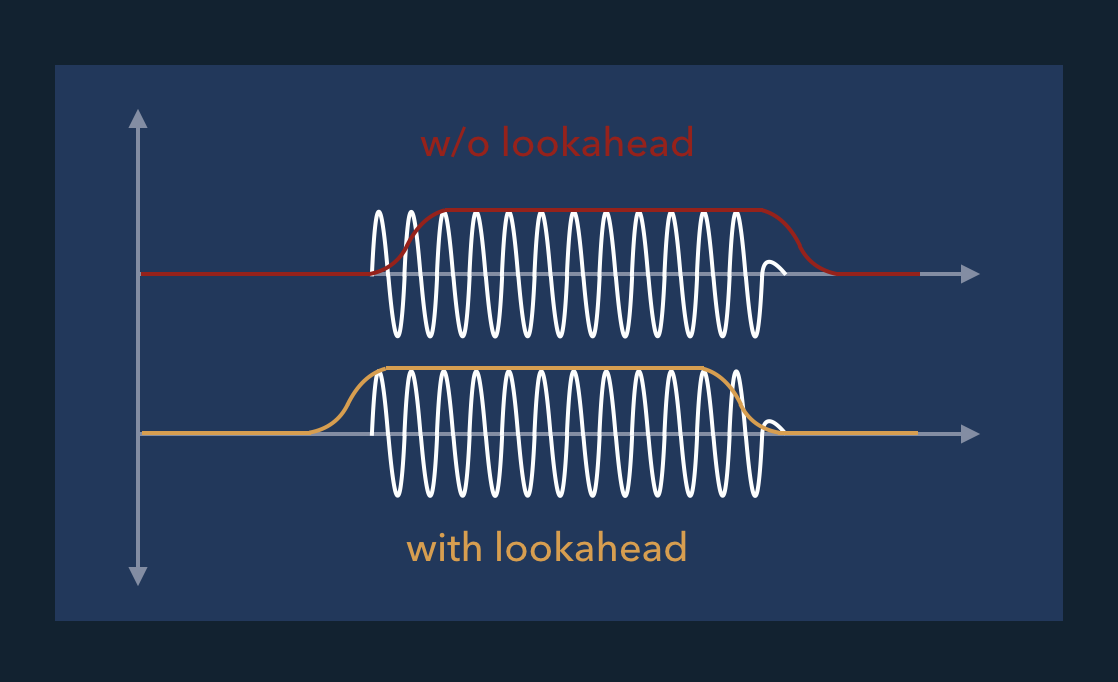
\includegraphics[width=\textwidth]{images/lookahead_w_o}
\caption{Gain adaption with and w/o lookahead}
\end{figure}

To achieve its goal the plug-in is designed to react slow and therefore needs some time adapt on a change in the average signal level. If it multiplies every sample with the gain value calculated form the same sample, the plug-in will be adjusted after the RMS has changed to the new average and the smoothed gain has slowly adapted. This will take some ms and consequently the first part of the alternate signal is not perfectly gained. While in particular this part introduces a new section in a song for example a chorus, it is desirable to have an adapted gain already at this point.\\
To compensate the adaption time I implemented a simple lookahead feature which allows the plug-in to calculate the gain for the current samples while looking at future samples.  This is realised by a ring buffer with two pointers at different locations. One write pointer to write the current sample transferred from the DAW into the buffer which is also used to determine the gain adaption and one read buffer ahead of it which is pointing on the sample that will be multiplied with the determined gain. To make this possible the gap between both pointers is as large as the set samples of the lookahead (converted from ms) and filled with zeros at the initialisation of the plug-in. In order to avoid that the whole plug-ins output is delayed I use the setLatencySamples()(see code besipel) method from JUCE to  communicate the resulting delay with the embedding DAW. Therefore a correct woking DAW will send the signal earlier to the plug-in and the output remains at the correct position despite the lookahead.\\
For the development I realised a fader in the UI to adjust the lookahead at runtime but in the final build the amount of samples is constant as I want the plug-in to be as simple to work with as possible. naja und weil ichja gewählt habe aus grund:

\begin{figure}[H]
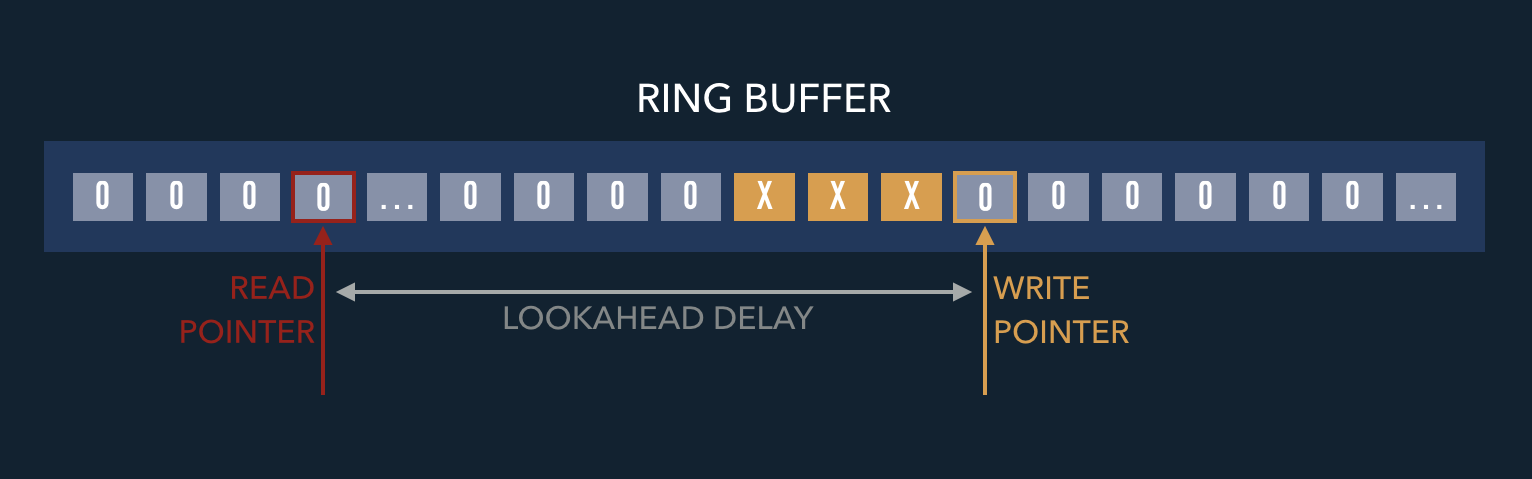
\includegraphics[width=\textwidth]{images/ring_buffer}
\caption{Initialized ring buffer with read and write pointers}
\end{figure}

vocals wichtig am Anfang erster push sollte nicht leiser gemacht sein weil vorher laut war oder andersrum
finale größe von delay sagen LOL
sollte nicht größer als ums sein oder
verweise zu den Bildern und code

\begin{lstlisting}[frame=single]
...
gain[channel] = updateGain(updateGate(rms2[channel], newGate),
gain[channel]);
double g = pow(10, gain[channel]/20);
delayData[dpw] = channelData[sample];
...
const double o = delayData[dpr] * g;
...
channelData[sample] = o;
...
if (++dpr >= delayBufferLength)
	dpr = 0;
if (++dpw >= delayBufferLength)
	dpw = 0;
...
\end{lstlisting}

\begin{lstlisting}[frame=single]
void AutoVocalCtrlAudioProcessor::updateDelay()
{
    int delayInSamples = msToSamples(*delayLength);
    delayReadPos = (int)(delayWritePos - delayInSamples
    + delayBufferLength) % delayBufferLength;
    setLatencySamples(delayInSamples);
}
\end{lstlisting}